\subsection{Indexing of Sub-Range Distributions}
\label{sec:blockhist_coding}
%%
We propose to index the sub-range distributions in such a way that the indexed distributions lead to even more space saving under any standard compression algorithm. In essence, the set of sub-range distributions, denoted by $B$, is indexed by a much smaller set of template distributions, denoted by $T$, which represents different types of distributions in the dataset. The proposed algorithm finds a mapping $\Theta: B \to T$ from each element $h_i(B)$ of $B$ to one or more elements of $h_j(T)$ of $T$. At the end, $B$ is discarded; only the map and the template set is retained. Since $B>>T$, this reduces the storage cost. In the query phase, the required elements of $B$ are approximated using the map and their images in $T$. Figure~\ref{fig:indexing_overview} presents a schematic overview of the indexing algorithm.
%%
%%%%%%%%%%%%%%%%%%%
%% Diagram begins
%%%%%%%%%%%%%%%%%%%
\begin{figure}[tb]
\centering
	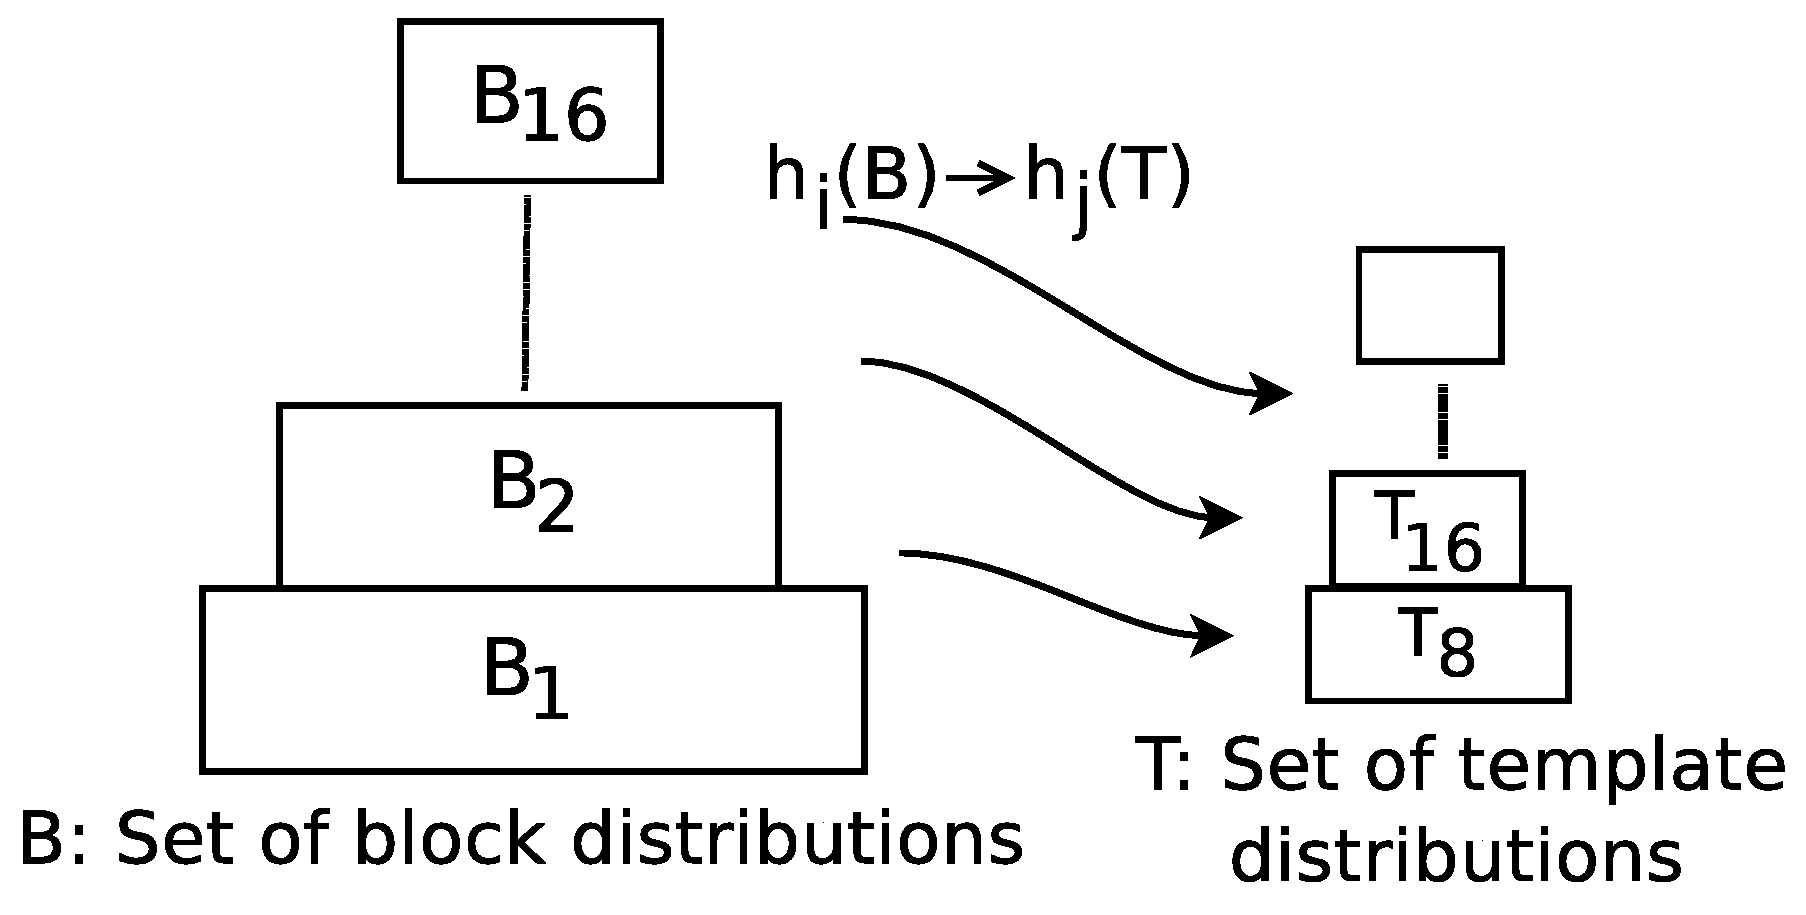
\includegraphics[width = 0.55\linewidth, keepaspectratio = true]{images/eps/indexing.eps}
	\caption{Overview of the indexing algorithm, where sub-range distributions, grouped based on their sizes, find an approximate match from a much smaller set of template distributions.}	
	\label{fig:indexing_overview}	
\end{figure}
%%%%%%%%%%%%%%%%%%%%
%% Diagram ends
%%%%%%%%%%%%%%%%%%%

A template based indexing performs well if the elements of $B$ are similar to each other so that many of them are indexed to one template. This reduces the number of elements to retain from $T$ and hence, reduces the total storage cost. In our case, the created sub-range distributions can be grouped based on the sizes of the blocks they come from, as shown by $B_1$, $B_2$ etc. in Figure~\ref{fig:indexing_overview}. The distributions of any given group $B_i$ are more likely to be similar to each other, which makes them easier to index against a certain type of templates. An integral distribution volume in its original form would not offer this benefit, since every distribution would come from a different-sized block. The steps of the indexing algorithm are described below. 

%%
%%
\subsubsection{Construction of Templates}
\label{subsec:templateconstruction}
%%
%The proposed algorithm works under the assumption that the data has redundancy and every feature (in our case distribution) has multiple copies in the data. Under this assumption, even if we select a few templates via regular sampling of the spatial domain, the likelihood of every type of distribution being selected at least once is high. This assumption also precludes the need to use expensive clustering methods for template creation, and hence suits large-scale data.
%%
%%%%%%%%%%%%%%%%%%%
%% Diagram begins
%%%%%%%%%%%%%%%%%%%
%\begin{figure}[tb]
%\centering
%	\includegraphics[width = 0.35\linewidth, keepaspectratio = true]{images/eps/templates_stratified.eps}
%	\caption{{\bf *** FIGURE WILL CHANGE ***}Proposed strategy for template creation. In this example, $H(P_1), \ldots H(P_9)$ - the normalized integral histograms at the sampled points - constitute the set of templates.}	
%	\label{fig:templatecreation}
%\end{figure}
%%%%%%%%%%%%%%%%%%%
%% Diagram ends
%%%%%%%%%%%%%%%%%%%

In our formulation, the distributions to be encoded (set $B$) come only from power-of-2 length blocks. This is why we create a similar structured yet much smaller set of templates $T$ from power-of-2 length blocks obtained from a downsampled copy of the data. Spatially smoothed downsampled data is used so that the local features and noises do not bias the templates. The templates are created using the following steps:
%%
\begin{packed_enumerate}
%%
\item The data is downsampled by one level using a standard spatial smoothing technique. We have an empty set $T$.
\item The downsampled data domain is decomposed into non-overlapping partitions of length $b$ where $b$ is a power of two. We have started with 4 as the initial value of $b$. 
\item Every $k$-th partition along each dimension is selected (where $k$ denotes stride) and its distribution is included in a set $T_b$
\item $T = T \bigcup T_b$
\item $b = 2\times b$ and $k = max \{k/2, 1\}$. Steps 2 and 3 are repeated with a bigger partition and a smaller stride. This is done until partition size is nearly half as the domain
%%
\end{packed_enumerate}
%%
This algorithm produces $T$ only from power-of-two blocks of different sizes. This makes it fit for indexing the hierarchy of block distributions $B$. Even though a sub-range distribution is free to index against any template coming from any region in the spatial domain, it is more likely to find a match from the subset coming from sub-ranges of equivalent size in the downsampled data. 
%%
%%
\subsubsection{Mapping Distributions to Templates}
\label{subsec:encoding}
%%
The next step is to create the map $\Theta: B\to T$. For each block histogram, the goal is to find a template which best approximates it. However, since $|T|<<|B|$, a block histogram may not find a good match in $T$. Thus, given an input block histogram, each template undergoes a set of transformations to virtually expand the set of templates available for each block. The proposed indexing can be expressed as following:
%%
\begin{align*}
\Theta(h_i(B)) = \{ j, \tau \}
\text{, if } \Delta(h_i(B),\tau(h_j(T)) \text{is minimum} \forall j
\end{align*}
%%
where $\tau$ represents the transformation of a template and $\Delta(a,b)$ represents the difference between histograms $a$ and $b$, 
%%
%%%%%%%%%%%%%%%%%%%
%% Diagram begins
%%%%%%%%%%%%%%%%%%%
\begin{figure}[tb]
\centering
	\subfloat[Intuition behind circular shift and reflection.]{\label{fig:histtransformreason}
	\includegraphics[width = 0.3\linewidth, keepaspectratio = true]{images/eps/histtransform_justification.eps}}
	~
	\subfloat[Peak matching followed by local alignment]{\label{fig:histtransformdetail}
	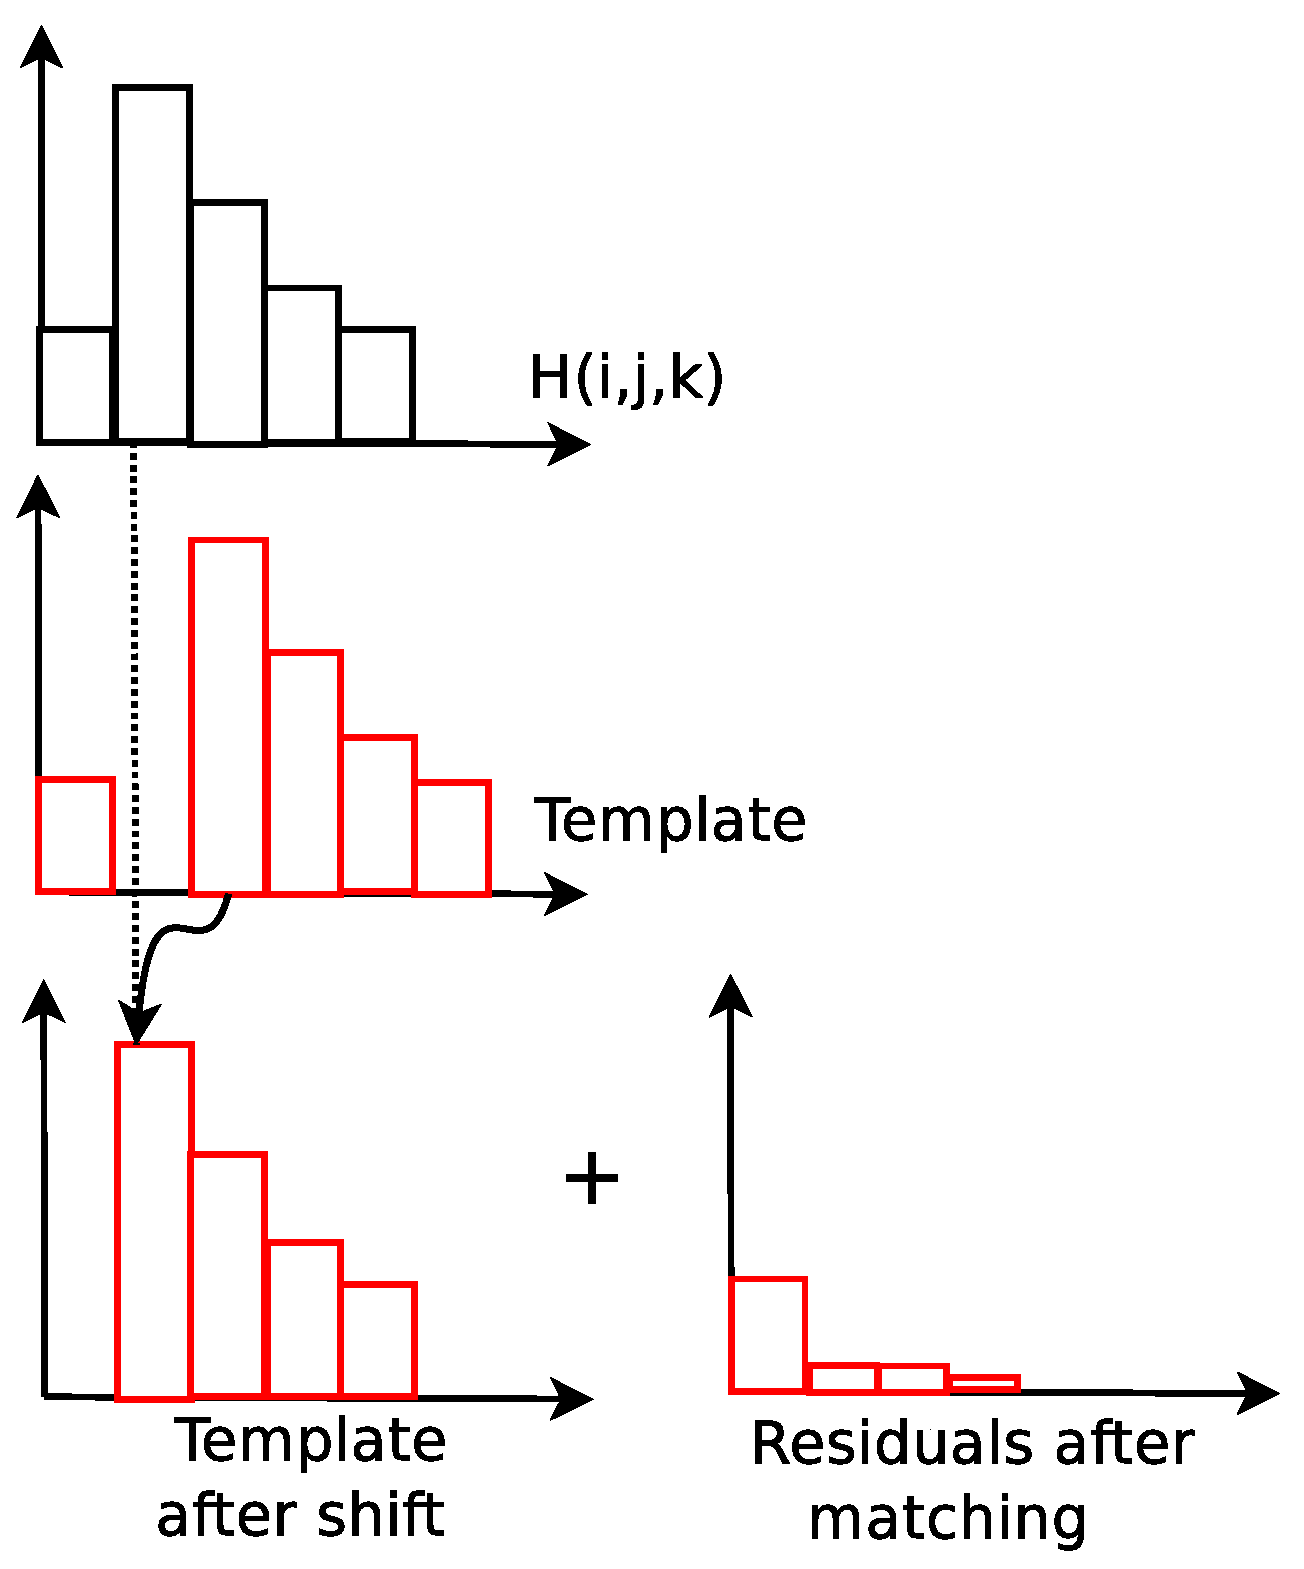
\includegraphics[width = 0.4\linewidth, keepaspectratio = true]{images/eps/histtransform_fast.eps}}
	\caption{(a) Schematic presentation of chosen transformations for histograms. (b) Fast implementation of shift and reflection through  peak matching and local adjustment.}	
	\label{fig:histtransform}
\end{figure}
%%%%%%%%%%%%%%%%%%%
%% Diagram ends
%%%%%%%%%%%%%%%%

We match histogram shapes by detecting corresponding points, which are the bin centers for a pair with same number of bins, and then transforming one to align the correspondent points. We observed that \emph{circular shift} and \emph{reflection} form a suitable set of aligning transformations. These two capture all possible shifts of the bins, while preserving the relative order. The intuition behind choosing these transformations is as follows:
%%
\begin{packed_itemize}
%%
\item Circular shift corresponds to change of location in the data space. In a volume data composed of multiple materials, when we move from one uniform zone $A$, made of one material, to another zone $B$ made of a different material, the data values shift and so does the histograms ($h(A)$ shifts to $h(B)$ as in Figure~\ref{fig:histtransformreason}). 
%%
\item Data sets also contain regions with gradually changing values. Change of location in such regions corresponds to reflection of histograms. For example, in Figure~\ref{fig:histtransformreason}, the histograms of $C$ and $D$ can be transformed though reflection followed by translation.
%%
\end{packed_itemize}
%%%
In case of a 1D histogram, the shifts are produced by shifting every bin to its right by one step at each iteration. The rightmost bin is circularly brought back to the leftmost bin. Then, if necessary, the histogram is reflected so that for each $i$, $f(i)$ becomes $f(K-i)$. Then $K$ circular shifts are applied on the reflected histogram. Instead of exhaustively matching against all shifted positions, we first align them by their mode (bin with highest frequency), and then shift the template only by a small number of steps in both directions ( Figure~\ref{fig:histtransformdetail} right). 

Under each of these transformations, the transformed template histogram is compared against the block distribution under consideration. After the input has been compared with all templates and all transformations, the $<$\emph{template,transformation}$>$ pair leading to minimum error ($\Delta$) is remembered. In our case, transformation $\tau (h)$ involves two pieces of information: the amount or rotation $n_R$, and a boolean flag $b_R$ denoting if reflection is needed. We measure error by L-2 norm, which is $\Sigma_{i=1}^K d_i^2$, where $d_i$ represents the difference between the frequencies at $i^{th}$ bins of two histograms under consideration. We also store the \emph{residuals} - bin-wise frequency differences between the block distribution and template chosen for it. 
%% 
%%
\subsubsection{Compression of Indexing Results}
\label{subsubsec:compression}
%%
The output of the above two steps is a $<$\emph{template,transformation, residual}$>$ triplet for each block distribution. It may be noted that, due to indexing, each of the three information has become friendly to compression. The template id can take values only within the range 0 to $(|T|-1)$, which is not large. The rotation amount can vary only between 0 and $(K-1)$, if $K$ bins are used. The reflection flag is only 0 or 1. Most importantly, the residuals are more likely to have very small numbers since the chosen template has already been aligned against the block distribution. 

Hence, each of these information can be stored in separate files and compressed using any off-the-shelf compression technique. We have experimented with a few lossless compression schemes such as LZ~\cite{lz77} and bzip2. However, our work is not tied up to any particular compression technique, we have focused on increasing the compressibility of the data in general.  